\documentclass[]{report}

\voffset=-1.5cm
\oddsidemargin=0.0cm
\textwidth = 480pt

\usepackage{framed}
\usepackage{subfiles}
\usepackage{graphics}
\usepackage{newlfont}
\usepackage{eurosym}
\usepackage{amsmath,amsthm,amsfonts}
\usepackage{amsmath}
\usepackage{color}
\usepackage{amssymb}
\usepackage{multicol}
\usepackage[dvipsnames]{xcolor}
\usepackage{graphicx}
\begin{document}

%------------------------------------------------------------------------------------------------%
\tableofcontents{3}

\section{Samples, Statistics and Parameters}


%-------------------------------------------------------%
\subsection{Sampling Error}
A random sample should be representative of the population. However, all statistics based on sample values, have an inherent sample value.
\\

A large sample provides more information about the population than a small sample so a statistic from a large sample will have less error.
\\ \bigskip
Suppose repeated samples are taken from the same population, and the same statistic (i.e. sample mean or sample variance) is calculated each time. These statistics will vary, which is to say, they have a distribution.

The probability distribution of a sample is called the \textbf{sampling distribution}.


\noindent \textbf{What is a Sample?}
A sample is a relatively small subset of people, objects, groups, or events, that is selected from the population. Instead of surveying every recent college graduate in the United States, which would cost a great deal of time and money, we could instead select a sample of recent graduates, which would then be used to generalize the findings to the larger population.


\begin{itemize}
\item A sample is a subset of a population.
\item Since it is usually impractical to test every member of a population, a sample from the population is typically the best approach available.
\end{itemize}

\noindent \textbf{Statistic}
\begin{itemize}
\item This is a numerical characteristic of the sample; a value
known when the sample is taken but that can change from sample to
sample.\\

\item In the clinical trial example, the statistic is the number of male
out the 30 individuals that respond well to the drug.
\end{itemize}






\noindent \textbf{Parameter}
\begin{itemize}
\item This is a numerical characteristic of the population; it is
a fixed number with an unknown value.\\ \vspace{0.2cm}
\item In the clinical trial example, the parameter could be the total
number of adult male that respond well to the drug. \vspace{0.2cm}
\end{itemize}



\begin{itemize}
\item Inferential statistics generally require that sampling be \textbf{random} although some types of sampling (such as those used in voter polling) seek to make the sample as representative of the population as possible by choosing the sample to resemble the population on the most important characteristics.
\end{itemize}

The major use of statistics is to use information from a \textit{\textbf{sample}} to infer something about a \textit{\textbf{population}}.
\begin{itemize}


\item A \textit{\textbf{population}} is a collection of data whose properties are analyzed. The population is the complete collection to be studied, it contains all subjects of interest.

\item A \textit{\textbf{sample}} is a part of the population of interest, a sub-collection selected from a population.

\item
A \textit{\textbf{parameter}} is a numerical measurement that describes a characteristic of a population, while a \textit{\textbf{sample statistic}} is a numerical measurement that describes a characteristic of a sample.

\item In general, we will use a statistic to infer something about a parameter. 
\end{itemize}



\subsection{Population}
\begin{itemize}
\item As is so often the case in statistics, some words have technical meanings that overlap with their common use but are not the same. Population is one such word. It is often difficult to decide which population should be sampled. 

\item For instance, if we wished to sample 500 listeners to an FM radio station specializing in music should the population be of listeners to that radio station in general, or of listeners to that stations classical music programme, or perhaps just the regular listeners, or any one of many other possible populations that you can construct for yourself? In practice the population is often chosen by finding one that is easy to sample from, and that may not be the population of first choice.

\item 
In medical trials (which are an important statistical application) the population may be those patients who arrive for treatment at the hospital carrying out the trial, and this may be very different from one hospital to another. If you look at any collection of official statistics (which
are most important for state planning) you will be struck by the great attention that is given to dening the population that is surveyed or sampled, and to the definition of terms. 


\item For instance, it has proved difficult to get consensus on the meaning of unemployed in recent years but a statistician must be prepared to investigate the population of unemployed. Think about this carefully.
\end{itemize}
\bigskip
\subsection*{Population}
\begin{itemize}
\item A population is a complete set of items that is being studied. It includes all members of the set. The set may refer to people, objects or measurements that have a common characteristic. Examples of a population are all high school students, all cats, all scholastic aptitude test scores.

\item A relatively small group of items selected from a population is a sample. If every member of the population has an equal chance of being selected for the sample, it is called a random sample. Examples of a sample are all algebra students at Central High School, or all Siamese cats.

\item Data are numbers or measurements that are collected. Data may include numbers of individuals that make up the census of a city, ages of pupils in a certain class, temperatures in a town during a given period of time, sales made by a company, or test scores made by ninth graders on a standardized test.

\item Variables are characteristics or attributes that enable us to distinguish one individual from another. They take on different values when different individuals are observed. Some variables are height, weight, age and price. Variables are the opposite of constants whose values never change.

\end{itemize}

\section{Systematic and Random Errors}
Experimental scientists make a fundamental distinction between \textbf{\emph{random}}, and
\textbf{\emph{systematic}} errors. To distinguish between random and systematic errors let
us consider a real experiment.\\

\noindent Four students (A-D) each perform an analysis in which exactly 10.00 $ml$
of exactly 0.1 M sodium hydroxide is titrated with exactly 0.1 NI
hydrochloric acid.
Each student performs five replicate titrations, with the results shown in
Table 1.1.

\begin{tabular}{|c|ccccc|l|}
\hline
% after \\: \hline or \cline{col1-col2} \cline{col3-col4} ...
Student & Results  & (ml) &  &  &  &Comment \\ \hline
A & 10.08 & 10.11 &10.09 &10.10&10.12 & Precise, biased\\ \hline
B & 9.88 &10.14& 10.02 &9.80& 10.21& Imprecise unbiased\\ \hline
C & 10.19 &9.79& 9.69 &10.05& 9.78 & Imprecise, biased\\ \hline
D & 10.04 &9.98 &10.02 &9.97 &10.04 & Precise, unbiased \\
\hline
\end{tabular}
\bigskip

\textbf{Graphical illustration}


The results of experiment represented by dot-plots. (The true value is 10.00).

%\begin{center}
%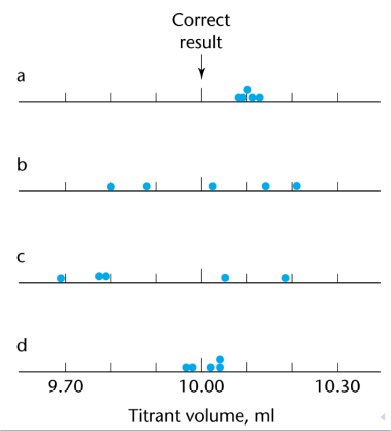
\includegraphics[scale=0.6]{Image10}
%\end{center}

Recall the average for each student $ 10.0950, 9.9600, 9.9300, 10.0025 $ respectively.


\textbf{Systematic error and bias}\\
Systematic error is a deviation of all measurements in one direction from the true value. It is well represented by the difference between the average value of the determined values and the true value
of the measured quantity. This difference is called the bias of measurements.

\textbf{Random error and precision}\\
Random error is a deviation of a measurement from the average of measured values.
It is well represented by the standard deviation of measurements.
This value is often called precision of measurements.

\textbf{Combined error vs. accuracy}\\
Accuracy is in inverse relation to the total deviation of a single measurement from the true value.


\subsection*{Definitions}
The key terms used in data collection can be defined as follows:
\begin{itemize}
\item A variable is the phenomenon being measured in the experiment or observational
study.
item A continuous variable takes any value on a range of real numbers.
item A discrete variable takes only distinct values, usually often integers (analogous to
‘counting’)
\end{itemize}


\subsection{Bias}
In addition to the common-sense meaning of bias, there is also a more technical meaning for the
word in statistics. This will be found both in Chapter 10 of this guide and in the work on estimators
in Statistics 2. It seems natural enough to wish to avoid bias, but it is not helpful to be swayed by
the value judgements inherited from the use of a word outside the limits of academic discussion.


\subsection*{Definitions of Statistical Terms}

Statistics is a branch of mathematics in which groups of measurements or observations are studied. The subject is divided into two general categories \textit{\textbf{ descriptive statistics}} and \textit{\textbf{inferential statistics}}. In descriptive statistics one deals with methods used to collect, organize and analyze numerical facts. Its primary concern is to describe information gathered through observation in an understandable and usable manner. 

Similarities and patterns among people, things and events in the world around us are emphasized. Inferential statistics takes data collected from relatively small groups of a population and uses inductive reasoning to make generalizations, inferences and predictions about a wider population.
Throughout the study of statistics certain basic terms occur frequently. Some of the more commonly used terms are defined below:


\subsubsection*{Populations and Samples}
\begin{itemize}
\item The collection of everyone or everything that is to be analyzed in a study is called a \textbf{population}. As we have seen in the examples above, the population could be enormous in size. There could be millions or even billions of individuals in the population. But we must not think that the population has to be large. If our group being studied is fourth graders in a particular school, then the population consists only of these students. Depending on the school size, this could be less than a hundred students in our population.

\item 
To make our study less expensive in terms of time and resources, we only study a subset of the population. This subset is called a \textbf{sample}. Samples can be quite large or quite small. In theory one individual from a population constitutes a sample. Many applications of statistics require that a sample have at least 30 individuals.
\end{itemize}
\subsubsection*{Parameters and Statistics}

The main objective of Statistics as a science is to estimate a population parameter by use of sample statistics.

What we are typically after in a study is the \textbf{parameter}. A parameter is a numerical value that states something about the entire population being studied. For example, we may want to know the mean wingspan of the American bald eagle. This is a parameter, because it is describing all of the population.

\begin{itemize}
\item Parameters are difficult if not impossible to obtain exactly. On the other hand, each parameter has a corresponding \textbf{statistic} that can be measured exactly. A statistic is a numerical value that states something about a sample. To extend the example above, we could catch 100 bald eagles and then measure the wingspan of each of these. The mean wingspan of the 100 eagles that we caught is a statistic.

\item The value of a parameter is a fixed number. In contrast to this, since a statistic depends upon a sample, the value of a statistic can vary from sample to sample. Suppose our population parameter has a value, unknown to us, of 10. One sample of size 50 has corresponding statistic with value 9.5. Another sample of size 50 from the same population has corresponding statistic with value 11.1.
\end{itemize}


\subsubsection*{Examples of Parameters and Statistics}

Below are some more example of parameters and statistics:

Suppose we study the population of dogs in Kansas City. A parameter of this population would be the mean height of all dogs in the city. A statistic would be the mean height of 50 of these dogs.
We will consider a study of high school seniors in the United States. A parameter of this population is the standard deviation of grade point averages of all high school seniors. A statistic is the standard deviation of the grade point averages of a sample of 1000 high school seniors.

\subsubsection*{Mnemonic Device}

There is a simple and straightforward way to remember what a parameter and statistic are measuring. All that we must do is look at the first letter of each word. A parameter measures something in a population, and a statistic measures something in a sample.

\section{Systematic and random errors}
Experimental scientists make a fundamental distinction between \textbf{\emph{random}}, and
\textbf{\emph{systematic}} errors. To distinguish between random and systematic errors let
us consider a real experiment.\\

\noindent Four students (A-D) each perform an analysis in which exactly 10.00 $ml$
of exactly 0.1 M sodium hydroxide is titrated with exactly 0.1 NI
hydrochloric acid.
Each student performs five replicate titrations, with the results shown in
Table 1.1.



\textbf{Systematic error and bias}\\
Systematic error is a deviation of all measurements in one direction from the true value. It is well represented by the difference between the average value of the determined values and the true value
of the measured quantity. This difference is called the bias of measurements.

\textbf{Random error and precision}\\
Random error is a deviation of a measurement from the average of measured values.
It is well represented by the standard deviation of measurements.
This value is often called precision of measurements.

\textbf{Combined error vs. accuracy}\\
Accuracy is in inverse relation to the total deviation of a single measurement from the true value.


\subsection{Sampling Techniques}
\begin{itemize}
\item Stratified Sampling
\item Random Sampling
\item Quota Sampling
\end{itemize}




\subsection{Random Sampling}
Random sampling is a sampling procedure by which each memmber of a population has an equal chance of being selected for a sample.

what does statistical inference refer to? Estimation and hypothesis testing

what are the names of the descriptive characteristics of populations and samples? paramaters and statistics respecgtively. In statistics, inferences are made about parameters by analysing their corresponding statistics.

How can representative samples be obtained? by random sampling.
%---------------------------------------------------------------%

\subsection{Random Sampling}
Though it may be clear that random sampling should avoid a sample biased
by the prejudices of the sampler, you should think carefully whether that is always a good idea.
In other times it was thought that a sampler could produce a better sample by using personal
judgement than by randomizing, because all the relevant facts could be taken into consideration.

Randomization is popular because this belief seems to be contradicted by experience. Remember
that a random sample may (though not very often) come out to look very biased just by chance
should one then reject it and try again? If the population has both men and women, would you
accept a random sample that just by chance included only men? 
\begin{itemize}
\item These difficulties are usually dealt
with by some form of restricted randomization. One might, for instance in the example above, use
a stratified random sample and select half the sample from the men and half from the women.
\item  To
carry out a random sample one needs a sample frame. This is the list of all the population units.
\item For instance, if you want to investigate UK secondary schools, the sample frame would be a list
of all the secondary schools in the UK. The key advantages of random sampling are that it avoids
systematic bias and it allows an assessment of the size of sampling error.

\item Random sampling is carried out, for many populations, by choosing at random without replacement
a subset of the very large number of units in the population. 
\item If the sample is a small proportion of
the population, then there is no appreciable difference between the inferences possible for sampling
with replacement and sampling without replacement.

\end{itemize}

\normalsize
\subsection{Cluster Sampling}

\begin{itemize}
\item \textbf{Cluster sampling} is a sampling technique that generates statistics about certain populations. 
\item Cluster sampling has a specific format required to obtain an appropriate sample, and though this sampling can help accurately gauge some information, it is not thought as accurate as simple random samples, where all groups of the same size have the same exact chance of being selected.
\end{itemize}
\normalsize




Cluster sampling is very popular on big voting nights. A natural division exists between voter precincts. By choosing some of the precincts and surveying or using exit polls at the chosen ones, there’s often a good sense what issues or what elected officials appear to be winning. The results of cluster samples are extrapolated to the entire population, and they’re often fairly representative of it. 




\begin{itemize}
\item The degree to which cluster sampling works tends to depend on what is being evaluated and how diverse of a population clusters represent.
\item  Suppose a statistician decided to break down voting precincts in a predominantly Republican state and create clusters of some of them to look for predictions about a national election.
\end{itemize}


These results would likely be skewed and not representative of the complete population in the US. On the other hand, cluster sampling with exit polling in a Republican or Democrat state could say a lot about the voting trends in the individual state. 

\subsection{Culster Sampling}

\begin{itemize}
\item \textbf{Cluster sampling} is a sampling technique that generates statistics about certain populations. 
\item Cluster sampling has a specific format required to obtain an appropriate sample, and though this sampling can help accurately gauge some information, it is not thought as accurate as simple random samples, where all groups of the same size have the same exact chance of being selected.
\end{itemize}

%-------------------------------------------------------------%

\subsection{Culster Sampling}
\begin{itemize}
\item Despite lacking the assurance that comes from using simple random samples or random samples, cluster sampling is used frequently in business and other applications. 

\item The basic procedure for creating cluster sampling is to divide the full population into some sort of meaningful groups. For instance, a fast foot restaurant might want a sense of what the most popular item ordered on their menu is. They might create a cluster/group for each McDonald’s store. They would then pick some of these clusters and obtain a sample from all people in that cluster. 
\item They could keep track of each customer’s order and decide which menu item is most popular or survey customers eating, but the company would only survey or track people in the chosen clusters; they’d also try to get all people at selected clusters. 

\end{itemize}




\normalsize
\subsection{Quota Sampling}

Quota sampling avoids the need for a sample frame. The interviewer seeks out units to ensure that
the sample contains given quotas of units meeting specied criteria (known as quota controls).
Quota sampling is cheap, but it may be biased systematically by the choices made by the inter-
viewer. For instance, interviewers avoid anyone who looks threatening, or too busy, or too strange.
Quota sampling does not allow an accurate assessment of sampling error.

\subsection{Stratified Sampling}

When people study statistics, they often find it challenging to remember the features of cluster sampling as opposed to the features of stratified sampling. The two have some similarities and key differences that are worth understanding. 


\begin{itemize}
\item In a stratified sample, a population is also divided into groups, though number of groups tends to be smaller. \item Population could be divided by gender, age, income, and region in which they live, and comparing the result of each group may be part of the reason the stratified sample is performed. 
\end{itemize}


\begin{itemize}
\item The huge and appreciable difference between stratified and cluster sampling is that when the groups are created, some members from each group or strata are selected. 
\item With a cluster, when clusters are created, the whole population of some of the clusters are used. 
\end{itemize}



\subsection{Stratified Sampling}
\begin{itemize}
\item A stratified sample is a mini-reproduction of the population. Before sampling, the population is divided into characteristics of importance for the research. For example, by gender, social class, education level, religion, etc. Then the population is randomly sampled within each category or stratum. If 38\% of the population is college-educated, then 38\% of the sample is randomly selected from the college-educated population.

\item In a stratified sample the sampling frame is divided into non-overlapping groups or strata, e.g.
geographical areas, age-groups, genders. A sample is taken from each stratum, and when this
sample is a simple random sample it is referred to as stratied random sampling.
\end{itemize}
\normalsize

\noindent \textbf{Advantages}\\

\begin{itemize}
\item Stratification will always achieve greater precision provided that the strata have been chosen so
that members of the same stratum are as similar as possible in respect of the characteristic of
interest. 

\item The bigger the differences between the strata, the greater the gain in precision. For
example, if you were interested in Internet usage you might stratify by age, whereas if you were
interested in smoking you might stratify by gender or social class.

\item It is often administratively convenient to stratify a sample. Interviewers can be specifically trained
to deal with a particular age-group or ethnic group, or employees in a particular industry. The
results from each stratum may be of intrinsic interest and can be analysed separately.

\item It ensures better coverage of the population than simple random sampling.

\end{itemize}
\textbf{Disadvantages}\\
\begin{itemize}
\item Difficulty in identifying appropriate strata.
\item More complex to organise and analyse results.
\end{itemize}

%===============================================================================================%



\subsection{Type of Samples}
There are a variety of different types of samples in statistics. Each of these samples is named based upon how its members are obtained from the population. Below is a list with brief description of some of the most common statistical samples.


\begin{framed}
List of Sample Types

\begin{itemize}
\item \textbf{Random sample} – Here every member of the population is equally likely to be a member of the sample.
\item \textbf{Simple random sample} – Not only is this a random sample, but every group of n is equally likely to be the sample.
\item \textbf{Voluntary response sample} – Here subjects from the population determine whether they will be members of the sample or not.
\item \textbf{Convenience sample} - This type of sample is characterized by the selection of easy to obtain members from the population.
\item \textbf{Systematic sample} - A systematic sample is chosen on the basis of an ordered system.
\item \textbf{Cluster sample} – A cluster sample involves using a simple random sample of evident groups that the population contains.
\item \textbf{Stratified sample} - A stratified sample results when a population is split into at least two non-overlapping subpopulations.
\end{itemize}
\end{framed}

It is important to know the distinctions between the different types of samples. For example, a simple random sample and a systematic random sample can be quite different from one another. Some of these samples are more useful than others in statistics. 

A convenience sample and voluntary response sample can be easy to perform, but these types of samples are not randomized to reduce or eliminate bias.

It is also good to have a working knowledge of all of these kinds of samples. Some situations call for something other than a simple random sample. We must be prepared to recognize these situations.



%============================================%


\subsection{Stratified Sampling}

In a stratified sample the sampling frame is divided into
non-overlapping groups or strata, e.g. geographical areas,
age-groups, genders.  A sample is taken from each stratum, and
when this sample is a simple random sample it is referred to as
stratified random sampling.


\noindent \textbf{Advantages}
Stratification will always achieve greater precision provided that
the strata have been chosen so that members of the same stratum
are as similar as possible in respect of the characteristic of
interest.  The bigger the differences between the strata, the
greater the gain in precision.  For example, if you were
interested in Internet usage you might stratify by age, whereas if
you were interested in smoking you might stratify by gender or
social class.

It is often administratively convenient to stratify a sample.
Interviewers can be specifically trained to deal with a particular
age-group or ethnic group, or employees in a particular industry.
The results from each stratum may be of intrinsic interest and can
be analysed separately.

It ensures better coverage of the population than simple random
sampling.







\subsection*{What Is the Difference Between a Parameter and a Statistic?}

In several disciplines the goal is to study a large group of individuals. These groups could be as varied as a species of bird, college freshmen in the U.S. or cars driven around the world. Statistics is used in all of these studies when it is infeasible or even impossible to study each and every member of the group of interest. Rather than measuring the wingspan of every bird of a species, asking survey questions to every college freshman, or measuring the fuel economy of every car in the world, we instead study and measure a subset of the group.



\subsection{Sampling Frame}
\begin{itemize}
\item In statistics, a sampling frame is the source material or device from which a sample is drawn.[2] 
\item It is a list of all those within a population who can be sampled, and may include individuals, households or institutions.
%\item Importance of the sampling frame is stressed by Jessen and Salant and Dillman.


\item Quota sampling is a non-probability sampling technique wherein the assembled sample has the same proportions of individuals as the entire population with respect to known characteristics, traits or focused phenomenon.
\end{itemize}





\subsection{Sampling}
Although it seems sensible to sample a population to avoid the cost of a total enumeration (or
census) of that population, it is possible to make a strong argument against the practice. One might
well consider that sampling is fundamentally unfair because a sample will not accurately represent
the whole population, and it allows the units selected for the sample to have more importance
than those not selected. This might be thought undemocratic. Many countries continue to take
a full census of their population, even though sampling might be cheaper. It is less obvious, but
true, that sampling might well be more accurate, because more time can be spent verifying the
information collected for a sample.



\subsection{Non-Sampling Error}

A statistical error caused by human error to which a specific statistical analysis is exposed. These errors can include, but are not limited to, data entry errors, biased questions in a questionnaire, biased processing/decision making, inappropriate analysis conclusions and false information provided by respondents.




\begin{itemize}
\item 
Non-sampling errors are part of the total error that can arise from doing a statistical analysis. 
\item The remainder of the total error arises from sampling error. 
\item Unlike sampling error, increasing the sample size will not have any effect on reducing non-sanpling error.
\item Unfortunately, it is virtually impossible to eliminate non-sampling errors entirely. 
\end{itemize}



\subsection{Sampling Error}

\begin{itemize}
\item A \textbf{statistical error} to which an analyst exposes a model simply because he or she is working with sample data rather than population or census data.
\item Using sample data presents the risk that results found in an analysis do not represent the results that would be 
obtained from using data involving the entire population from which the sample was derived.
\end{itemize}


\begin{itemize}
\item The use of a sample relative to an entire population is often necessary for practical or budgetary reasons. 
\item Although there are likely to be some differences between sample analysis results and population analysis results, the degree to which these can 
differ is not expected to be substantial. 
\end{itemize}



\begin{itemize}
\item Methods of reducing sampling error include increasing the sample size and ensuring that the sample adequately represents the entire population.
\end{itemize}

%---------------------------------------------------------------%

\newpage
\chapter{Sampling}


\subsection{Stratified Sampling}

When people study statistics, they often find it challenging to remember the features of cluster sampling as opposed to the features of stratified sampling. The two have some similarities and key differences that are worth understanding. 



%-------------------------------------------------------------%

\subsection{Cluster Sampling}

\begin{itemize}
\item The degree to which cluster sampling works tends to depend on what is being evaluated and how diverse of a population clusters represent.
\item  Suppose a statistician decided to break down voting precincts in a predominantly Republican state and create clusters of some of them to look for predictions about a national election.
\end{itemize}

%-------------------------------------------------------------%

\subsection{Cluster Sampling}

These results would likely be skewed and not representative of the complete population in the US. On the other hand, cluster sampling with exit polling in a Republican or Democrat state could say a lot about the voting trends in the individual state. 




%--------------------------------------------------------------------------------------%

\subsection{Cluster sampling }
Cluster sampling is a sampling technique that generates statistics about certain populations. It has a specific format required to obtain an appropriate sample, and though this sampling can help accurately gauge some information, it is not thought as accurate as simple random samples, where all groups of the same size have the same exact chance of being selected. 

%--------------------------------------------------------------------------------------%
%--------------------------------------------------------------------------------------%

When people study statistics, they often find it challenging to remember the features of cluster sampling as opposed to the features of stratified sampling. The two have some similarities and key differences that are worth understanding.

%--------------------------------------------------------------------------------------%
%--------------------------------------------------------------------------------------%

\subsection{Stratified Sampling}
The degree to which cluster sampling works tends to depend on what is being evaluated and how diverse of a population clusters represent. Say a statistician decided to break down voting precincts in a predominantly Republican state and create clusters of some of them to look for predictions about a national election. These results would likely be skewed and not representative of the complete population in the US. On the other hand, cluster sampling with exit polling in a Republican or Democrat state could say a lot about the voting trends in the individual state.

%--------------------------------------------------------------------------------------%

%==============================================================================================%


We will never find out these values unless we ask everyone in the population. The value of a parameter is fixed but usually unknown. We estimate it by using information from a sample. 

Statistic: this represents some value (e.g. an average value or a percentage) that we are interested in calculating for the sample for example the percentage of a representative sample of adults who will vote for a particular political party or the average age of this representative sample. 

%==============================================================================================%

\begin{itemize}
\item We can find out these values since we can ask everyone in the sample but if we took a different sample of people we might get a different answer. The value of a statistic is not fixed but is known. 

\item We estimate the value of the parameter by using the value of the statistic.
\end{itemize}

%==============================================================================================%

\subsection{Example}

A telesales company in Cork uses a device that dials residential phone numbers in the city at random. Of the first 100 numbers dialed, 7 are unlisted.  10\% of all Cork residential phones are unlisted. Is the 7\% a statistic or a parameter? Is the 10\% a statistic or a parameter?



%==============================================================================================%


%- Example 1 Telesales Company[pg7]

The 7\% value is a statistic because it is a value based on a sample.

The 10\% value is a parameter value because it is based on all members of the populations  (i.e. all residential numbers in Cork)


A T.D. is interested in whether her constituents are in favour of the new government tax on plastic bags. Her staff reports that letters on the issue have been received from 300 constituents and that 200 of these are in favour of the tax. Identify the population, variable measured and the sample. 




%==============================================================================================%
%- Example 2 Plastic Bag tax survey[pg7]

Population : All of the TDs Constituents

Variable measured: Whether or not a constituent is in favour of the plastic bag tax

Sample : The 300 respondents to the survey






%==============================================================================================%

%- 1.4.2 

\section{Non-probability Sampling Methods}
Sampling methods are the different ways of selecting a subset of individuals from the population. We can select a group simply because it’s easy for us to contact these people and they are willing to answer our questions. This method of sampling is appropriately called convenience sampling. The sample is identified primarily by convenience e.g. volunteer panels for consumer research. The advantage is relatively easy sample selection and data collection but it is impossible to evaluate the “goodness” of the sample in terms of its representativeness of the population.

We can also use an “expert” to pick the people he or she considers most representative of the population. This is called judgement sampling. The quality of the sample depends on the judgement of the person selecting it.

%==============================================================================================%

Quota sampling is another method of sampling widely used in opinion polling and market research. Interviewers are each given a quota of subjects of a specified type to survey for example, an interviewer might be told to find 20 adult men and 20 adult women, 10 teenage girls and 10 teenage boys to interview about their television viewing. 

%==============================================================================================%

\begin{itemize}
\item It is clear that these methods are open to mistakes being made. Let’s go back to the example of the pre-election poll on who is going to win the election. 
\item If I pick a group of people to answer this question simply because it’s convenient for me, my sample may include all people from a particular background and exclude everyone from a different background. Can I be certain that the conclusions for these people can be applied to the whole population? 

\end{itemize}


%==============================================================================================%
\newpage
%%- 1.4.4  
\section*{Probability Sampling Methods}

All methods of sampling based on taking a random sample are called probability sampling methods since we know the chance (or probability) of someone getting into our sample i.e. it is the same for everyone. Convenience, judgement and quota sampling methods are called non-probability sampling methods since we don’t know what the chances are for an individual getting into our sample i.e. it is not the same for everyone. Many methods of analysis make the assumption that the sample from which the data are collected is a random sample. 

%==============================================================================================%

\begin{itemize}
\item There are many different types of probability sampling. These include:

\item Stratified Random sampling: Stratified sampling techniques are generally used when the population is heterogeneous (dissimilar) and where certain homogeneous (similar) sub-populations can be isolated. 

\item These sub-populations are called strata. The population is divided into strata, such that each unit in the population belongs to one and only one stratum. The basis for forming the strata could be age, gender, industry type etc.  A simple random sample is taken from each stratum. 
\end{itemize}

%==============================================================================================%
\subsection*{Cluster Sampling}
Cluster sampling: the population is divided into separate groups of units called clusters. Each unit belongs to one and only one cluster. A simple random sample of clusters is selected from a list of all clusters. All units within each chosen cluster are included in the sample. 

%==============================================================================================%

\begin{itemize}
\item A cluster could be a housing estate or other well-defined area. Cluster sampling is typically used when a researcher cannot get a complete list of the members of a population they wish to study but can get a complete list of groups or 'clusters' of the population. 
\item It is also used when a random sample would produce a list of subjects so widely scattered that surveying them would prove to be far too expensive, for example, people who live in different counties in Ireland. 
\end{itemize}

%==============================================================================================%
\subsection*{Systematic Sampling}
\begin{itemize}
\item Systematic sampling : For example, if a sample of size 50 is required from a population with 5000 units we would include in the sample one unit for every 5000/50 = 100 units in the population. One of the first 100 units of the population is selected at random from a list of all members of the population. 

\item Other sample units are found by starting with the first unit and then selecting every 100th unit that follows in the population list. 

\item In effect, the sample of 50 is identified by moving systematically through the population and identifying every 100th unit after the first randomly selected unit.
\end{itemize}


%==============================================================================================%
%==============================================================================================%

\subsection{Lack of precision in sampling }
A large random sample will include many people with lots of different characteristics whereas a small sample will not have the same range of people or characteristics. Thus, the results from one small sample may differ considerably from the results of another small sample depending on the range of people and characteristics it includes.
%% 1.3.5  Lack of precision in sampling 

Lack of precision is where the result of sampling is not repeatable. Every time we take a sample and ask the question of interest, we get a different answer. How can we make conclusions for the population if we get different answers from each sample? How can we correct this problem? If we increase the sample size, we also increase the repeatability or precision of our results. 



\subsection{Errors in Sampling}

\begin{itemize}
\item Sampling errors (related to the act of selecting the sample) e.g. biased sampling method; sampling frame which differs from the population

\item Non-sampling errors (not related to the act of selecting the sample) e.g. missing data, response errors, processing errors, wording of questions 
\end{itemize}







\end{document}
